\subsection{Classic Planning Formalism}
\label{sec:pddl_formalism}
In this section, we will describe the methods that follow the classic task-planning formalism. Before introducing the methods, it is crucial to define the formalism with a set of foundational definitions.

Task-planning is a well-known problem that has been studied for many years. One of the most influent formalizations, still widely used today, is STRIPS (Stanford Research Institute Problem Solver) \cite{fikes1971strips}, which was developed in the 70s. STRIPS was initially an automated planning solver, but its primary contribution lies in its definition of a planning problem, which has served as the foundation for much of the research in subsequent decades.

According to the STRIPS formalism, a planning task is defined as a tuple $\Pi = (P, A, s_0, G, c)$, where:
\begin{itemize}
    \item $P$ is a set of propositions (also called facts).
    \item $A$ is a set of actions.
    \item A state $s$ is a subset of predicates, $s \subseteq P$, where $s_0$ is the initial state,
    \item $G \subseteq s$ represents the goal conditions.
    \item $c: A \leftarrow R$ is the cost function, which assign to an anction $a \in A$ a real-value, $c(a)$ representing the cost of performing a given action.
\end{itemize}

An action $a \in A$ is defined as a tuple $a = \left(pre(a), add(a), del(a)\right)$, where $pre(a), add(a), del(a) \subseteq P$. These represent:
\begin{itemize}
    \item $pre(a)$: the preconditions (i.e., predicates that must be true to perform the action).
    \item $add(a)$: the added conditions (i.e., predicates that become true after the action is executed).
    \item $del(a)$: the deleted conditions (i.e., predicates that become false after the action is executed).
\end{itemize}
with the constraint that $add(a) \cap del(a) = \emptyset$. According to this formalism, an action is applicable in a state $s$ if $pre(a) \subseteq s$, and it results in the successor state $s' = (s \setminus del(a)) \cup add(a)$.

Building on these foundational concepts, the \textbf{Planning Domain Definition Language} (PDDL) was introduced in the 90s \cite{aeronautiques1998pddl}. PDDL is a human-readable format for describing automated planning problems. It provides a way to describe, the possible states of the world, the set of available actions, where each action description includes the prerequisites and the effects of the action, a specific initial state of the world and a specific set of desired goals. 

PDDL separates the model of a planning problem into two main components:
\begin{enumerate}
    \item The domain description, which defines the elements that are common across all problems within a given domain.
    \item The problem description, which specifies the specific planning problem, including the initial state and the goals to be achieved.
\end{enumerate}

\begin{figure}[t]
    \centering
    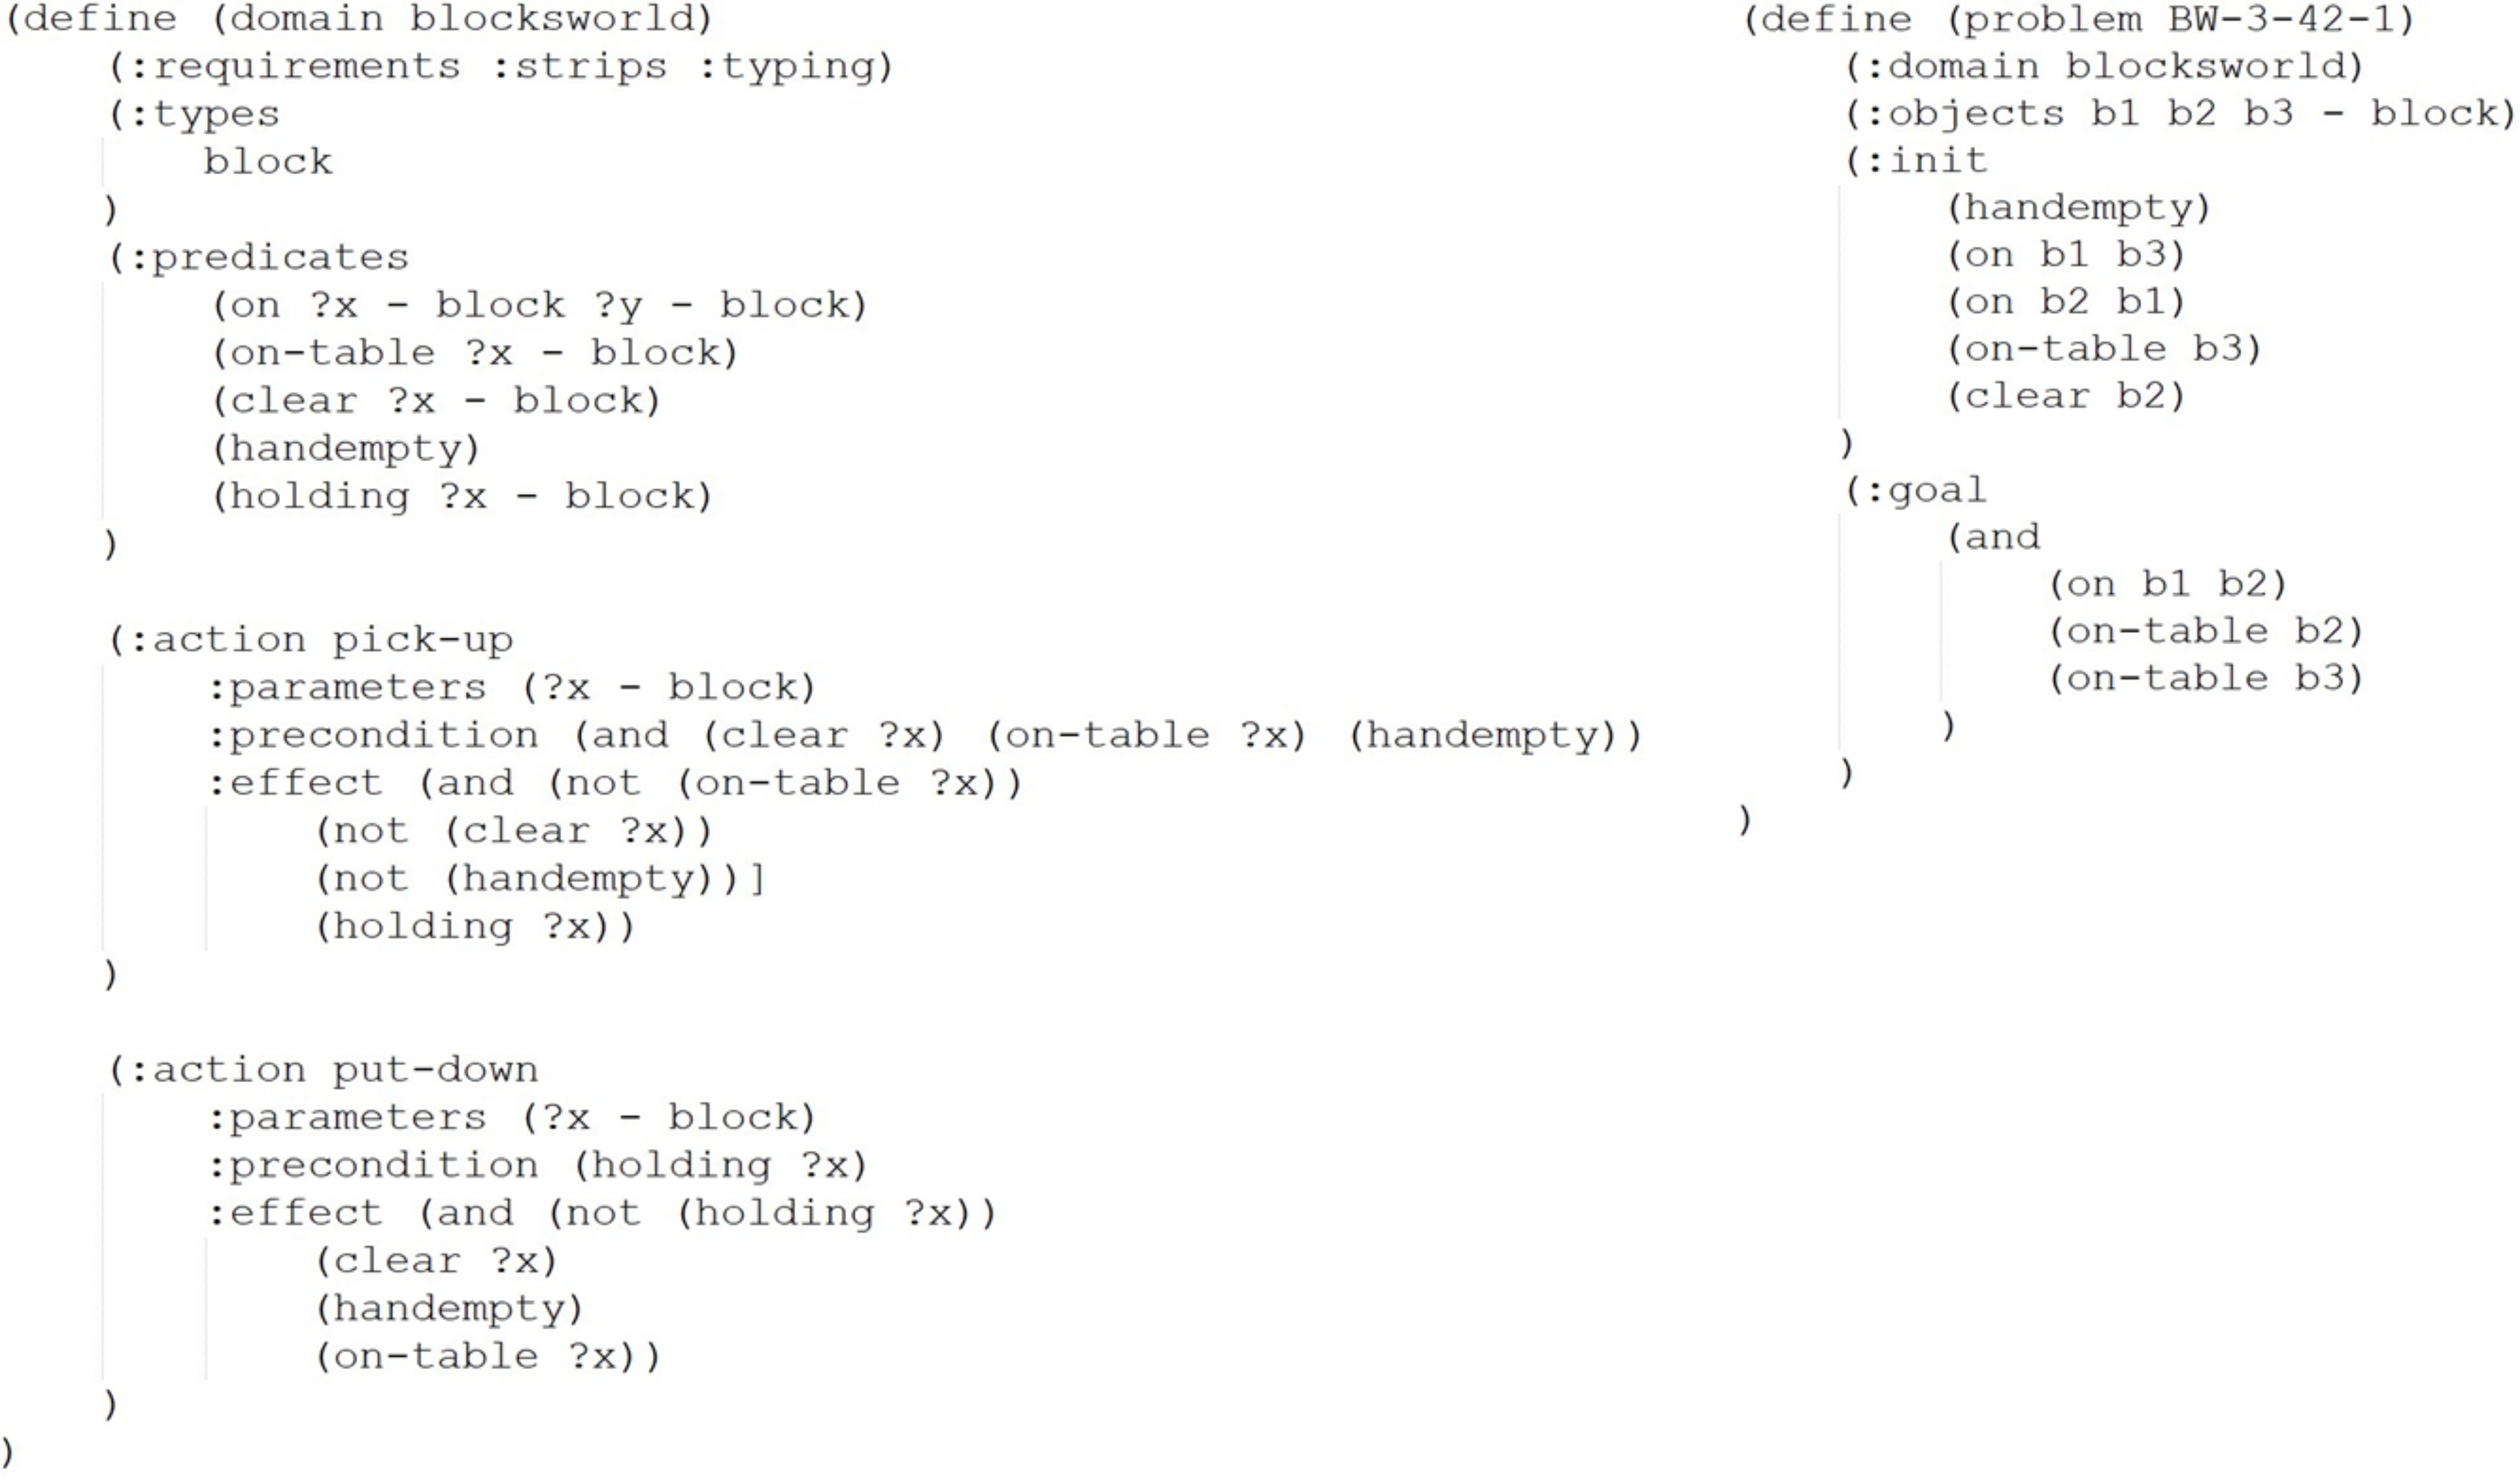
\includegraphics[width=1.0\textwidth]{figures/images/ch4/domain_problem.jpg}
    \caption{(Left) Example of a domain definition for the Blocks-World, specifying the predicates and actions available in the environment. (Right) Example of a problem definition for the domain, where a specific instance of the problem is defined, including object instances, the initial state, and the desired goal state.}
    \label{fig:domain_problem}
\end{figure}


Figure \ref{fig:domain_problem} provides examples of domain and problem definitions for the Blocks-World environment. As shown, when using the PDDL formalism, it is essential to fully define the elements of the world (e.g., blocks), the available actions (e.g., pick-up), along with their corresponding preconditions (i.e., predicates that must be true for the action to be executed) and postconditions (i.e., the effects of the actions). In the problem definition, specific instances of objects in the environment are specified, along with the initial state and goal state, both of which are defined based on the predicates available in the domain definition.

Once the problem is defined using the PDDL formalism, a complete parameterized instance must be specified to obtain a solution to the planning problem. This involves solving what is known as the \textbf{grounding problem}. During this process, all predicate and action variables must be instantiated with the objects defined in the problem. For instance, in the example shown in Figure \ref{fig:domain_problem}, the variable \( x \) is replaced with objects \( b1 \), \( b2 \), and \( b3 \) from the problem definition, leading to a complete enumeration of all predicates and actions. The result of this process is known as the \textit{Grounded Planning Problem}, which follows the same formalism as the STRIPS representation described earlier.

The grounded problem then serves as the input for planning algorithms, such as the well-known Fast Downward \cite{helmert2006fast} or LAMA \cite{richter2010lama}. While delving into the specifics of these algorithms is beyond the scope of this section, it is crucial to note that they are essentially \textit{search algorithms}. Given a state-space represented as a graph, which is derived from the Grounded STRIPS representation, these algorithms compute the (estimated) shortest path in the state-space, connecting the source node (representing the initial state) to the target node (representing the goal state).

The limitations of these approaches have been well-known for a long time. Specifically, these algorithms do not scale well as the size of the problem (in terms of actions, predicates, and objects) increases. There are two main areas where higher problem dimensionality can cause performance issues:

\begin{enumerate}
    \item \textit{Search Phase}, as the dimensionality of the problem increases, the state-space expands correspondingly. This increases the time required to explore the state-space and find a solution path.
    \item \textit{Grounding Problem}, as the problem dimensionality grows, the time needed to generate a complete enumeration of all object combinations grows exponentially.
\end{enumerate}

To address the first issue, research has focused on developing methods to accelerate the search phase by introducing \textit{heuristics} that guide the search more efficiently towards the goal state. For the second issue, the literature has proposed methods that perform \textit{partial} grounding, concentrating on the action instances that are most relevant to the specific problem instance. Examples of these methods will be discussed in the following two paragraphs.

Here, a heuristic is a function $h: S \rightarrow \mathbb{R}$, which maps a state $s \in S$ to a real value $h(s)$, representing an estimate of the cost to reach the goal state from the state $s$. The optimal heuristic, denoted $h^{*}(s)$, is the heuristic that gives the exact cost of the optimal plan to reach a goal state from $s$. A heuristic is considered \textit{admissible} if it never overestimates the actual cost, i.e., $h(s) \leq h^{*}(s), \forall s \in S$. By utilizing the heuristic cost, a search algorithm can focus on exploring the most promising states instead of performing an exhaustive search of the entire state space.

In the context of task planning, a common heuristic is computed by solving the \textbf{Relaxed-STRIPS} problem. This is a simplified version of the STRIPS problem, where the delete conditions ($del$) are ignored, i.e., an action $a$ is represented as $a = \left(pre(a), add(a), \emptyset \right)$. The Relaxed-STRIPS problem is easier to solve because removing the $del$ conditions relaxes some of the constraints, allowing the state to include predicates that logically cannot be true simultaneously. By solving this relaxed problem, an estimated cost for reaching the goal from a given state can be computed. This approach has been used in well-known algorithms such as Fast-Downward \cite{helmert2006fast} and combined with novel heuristics in LAMA \cite{richter2010lama}.

\paragraph*{Heuristic Estimation}\mbox{}\\
In this paragraph the methods that methods that propose GNN for computing heuristics estimation through the usage of GNNs are discussed. Specifically, the review will focus on two recent works \cite{shen2020learning,chen2024learning}.

The first remarkable work towards the use of GNN for heuristic estimation was proposed by authors of \cite{shen2020learning}. Here, authors started from the idea to leverage data-driven approaches to learn an heuristic function, and explore the possibility of such methods to generalize to different cardinalities and problems, and comparing the performance of such methods with classic heuristic functions.

The first step to solve this problem is related to the definition of the input. Specifically, the authors started by the Relaxed-STRIPS formulation. The STRIPS problem can be easly formulated as a graph if the following observations are done:
\begin{itemize}
    \item A node, can be described a predicate which can be either a pre-condition or an added condition.
    \item The edge is represented by the action that connects the pre-conditions to the added-conditions. 
\end{itemize}
Figure \ref{} illustrates the mapping of predicates and actions to graph nodes and edges. As can be observed, an action connects multiple nodes. To model this, the authors use a generalized graph structure known as a \textit{hypergraph}. Formally, a hypergraph is defined as a triple $G = (u, V, E)$, where $V = \left\{ \textbf{v}_{i}: i \in \left\{1, 2, \dots, N^{v} \right\} \right\}$ is the set of $N^{v}$ vertices, and $E = \left\{ (e_{k}, R_{k}, S_{k}): k \in \left\{1, 2, \dots, N^{e} \right\} \right\}$ is the set of $N^{e}$ hyper-edges. In this structure, $R_{k}$ is the receiver set, containing the indices of the nodes for which the $k$-th edge acts as an incoming edge, and $S_{k}$ is the sender set, containing the indices of the nodes for which the $k$-th edge acts as an outgoing edge. Then, $\textbf{v}_{i}$ is the node embedding, which has been implemented as a binary-vector $v_i = [x_s, x_g]$, where $x_s, x_g \in \left\{0,1\right\}$. $x_s=1$ iff the i-th predicate is true in the state s and $x_g=1$ iff the predicate is true in the goal-state. While, $e_{k}$ is the edge embedding, $e_k = [c(a_k), |Pre(a_k)|, |Add(a_k)|]$, where $c(a_k)$ is the cost of the operator, $|Pre(a_k)|$ is the number of pre-condition and $|Add(a_k)|$ is the number of added condition.

Once the graph structure has been defined, the module that processes this input can be described. Specifically, the authors propose leveraging the concept behind the \textit{Interaction Network} \cite{battaglia2016interaction}. The architecture, depicted in Figure \ref{}, implements the computational flow shown in Figure \ref{}, and can be divided into the following three steps.
\smalltodo{add figure}

The \textit{Encoding Block} consists of two functions, $\phi^{e}$ and $\phi^{v}$, both implemented as Multi-Layer Perceptrons (MLPs). Specifically, $\phi^{e}(e_j) = e_{hid}^{0}$ and $\phi^{v}(v_i) = v_{hid}^{0}$, where $e_{hid}^{0}, v_{hid}^{0} \in \mathbb{R}^{32}$. This transformation expands a binary vector of size 2 or 3 into a vector of size 32, representing a weighted combination of MLP outputs, since the input is binary.

The \textit{Core Block} implements the Message-Passing Iterative Procedure, which is further broken down into the following steps:

\begin{enumerate}
    \item \textit{Edge Block}: For a given edge (action) $e_{hid,j}^{t-1}$, the embedding is constructed as defined in Equation \ref{equation:edge_input}. Here, $max-rec$ and $max-sen$ refer to the maximum number of receivers and senders, respectively. If an operator has fewer receivers or senders, zero-padding is applied. The message to be propagated is built using a shared MLP for each edge: $e_{hid,j}^{t} = \phi^{e}(e_{hid,j}^{t-1})$.
    \begin{equation}
        \begin{aligned}
            e_{hid, j}^{t-1} = \Big[ & e_{hid,j}^{0}, e_{hid,j}^{t-1}, \\
            & v_{hid,r_0}^{0}, \dots, v_{hid,r_{max-rec}}^{0}, \\
            & v_{hid,r_0}^{t-1}, \dots, v_{hid,r_{max-rec}}^{t-1}, \\
            & v_{hid,s_0}^{0}, \dots, v_{hid,s_{max-sen}}^{0}, \\
            & v_{hid,s_0}^{t-1}, \dots, v_{hid,s_{max-sen}}^{t-1} \Big]
        \end{aligned}
        \label{equation:edge_input}
    \end{equation}
    
    \item \textit{Node Block}: As in the Interaction Network, only the states of the receiver nodes are updated. The information from the operators affecting the receivers is aggregated by the function $\rho^{e \rightarrow v}$, which sums the incoming edges. The input to the node function is built as shown in Equation \ref{equation:node_input}, and the node embeddings are updated using a shared MLP for each node: $v_{hid,i}^{t} = \phi^{v}(v_{hid,i}^{t-1})$.
    \begin{equation}
        \begin{aligned}
            v_{hid, i}^{t-1} = \Big[ & \rho^{e \rightarrow v}(\left\{e_{hid,j}^{t} | e_j \text{ is an incoming edge} \right\}), \\
            & v_{hid,i}^{0}, v_{hid,i}^{t-1} \Big]
        \end{aligned}
        \label{equation:node_input}
    \end{equation}
    
    \item \textit{Global Block}: This block is responsible for updating the global representation of the graph. The node embeddings and edge embeddings are aggregated using the functions $\rho^{e \rightarrow u}$ and $\rho^{v \rightarrow u}$, respectively, both of which sum the embeddings. The new global representation is then obtained by applying an MLP.
\end{enumerate}

The operations in the core block are repeated for $M$ iterations, where $M = 10$ in this work.
The system is trained by minimizing the loss function defined in Equation \ref{equation:loss_func}. Here, $h^{*}(s)$ represents the ground truth heuristic value for state $s$, obtained by solving the training planning problem with a classical planning algorithm.
\begin{equation}
    \mathcal{L}_\theta(\mathcal{B})=\frac{1}{|\mathcal{B}|} \sum_{\left(G, h^*(s)\right) \in \mathcal{B}} \frac{1}{M} \sum_{t \in \{1, \ldots, M\}}\left(h_t^\theta(G)-h^*(s)\right)^2
    \label{equation:loss_func}
\end{equation}

To test the proposed architecture, the authors proposed to test it in different scenarios, using different domains. 


\paragraph*{Grounding Problem}\mbox{}\\

